\documentclass{article}
\title{some insight into consumer theory}
\author{Dawei Wang}
\date{\today}
\usepackage{ctex}
\usepackage{amsmath}
\usepackage{amssymb}
\usepackage{graphicx} %插入图片的宏包
\usepackage{float} %设置图片浮动位置的宏包
\usepackage{subfigure} %插入多图时用子图显示的宏包
\begin{document}
	\maketitle

\section{选择偏好与效用}

禀赋(endowment):是指一个消费者所拥有的一束商品,并可以用来与其他商品进行交换。禀赋定义的一个特征是:因为消费者拥有禀赋束,故其可以选择无视商品的市价消费掉那束商品。

当预算约束来自禀赋时,对消费者而言可获得的货币不是固定的。可得的货币取决于禀赋束中商品被赋予的价格。当禀赋束中的商品价格变化时预算线围绕禀赋点旋转。

个人思考:就个人发展而言我要做的就是提升自己的禀赋这样预算线就可以外移有更多选择。

\section{偏好}

单调性:越多越好(至少不更差),无差异曲线向下倾斜。

凸性: 对多样性的渴望,严格凸会导致递减的边际替代率。

\section{效用函数与偏好}

效用函数仅是对商品束进行配数的数学规则(对无差异曲线上的点的映射),要求对更加偏好的商品束分配较高的数。——某种意义上是对幸福的量化,效用在经济学理论中是作为消费者最优化自己选择的最高指导。

把表示同一效用大小的点(商品束)连起来就得到无差异曲线。

决定无差异曲线本质的是其形状和排序,因为不同消费者幸福本质上是无法比较的东西,马云多赚一个亿带来的幸福的提高显然不如普通老百姓多赚一个亿,这也是序数效用论取代基数效用论的原因。

若两个效用函数的MRS(斜率)相同、序相同,则其代表同一个偏好。(MU不需要相同,因其不决定形状和序)。

综上,保序变换也可以理解为不改变无差异曲线的形状和序的变换。(注:题目中涉及是否为单调变换的判断时有时需考虑定义域来讨论。)

\section{不同类型的偏好}



\begin{figure}[H] %H为当前位置,!htb为忽略美学标准,htbp为浮动图形
	\centering %图片居中
	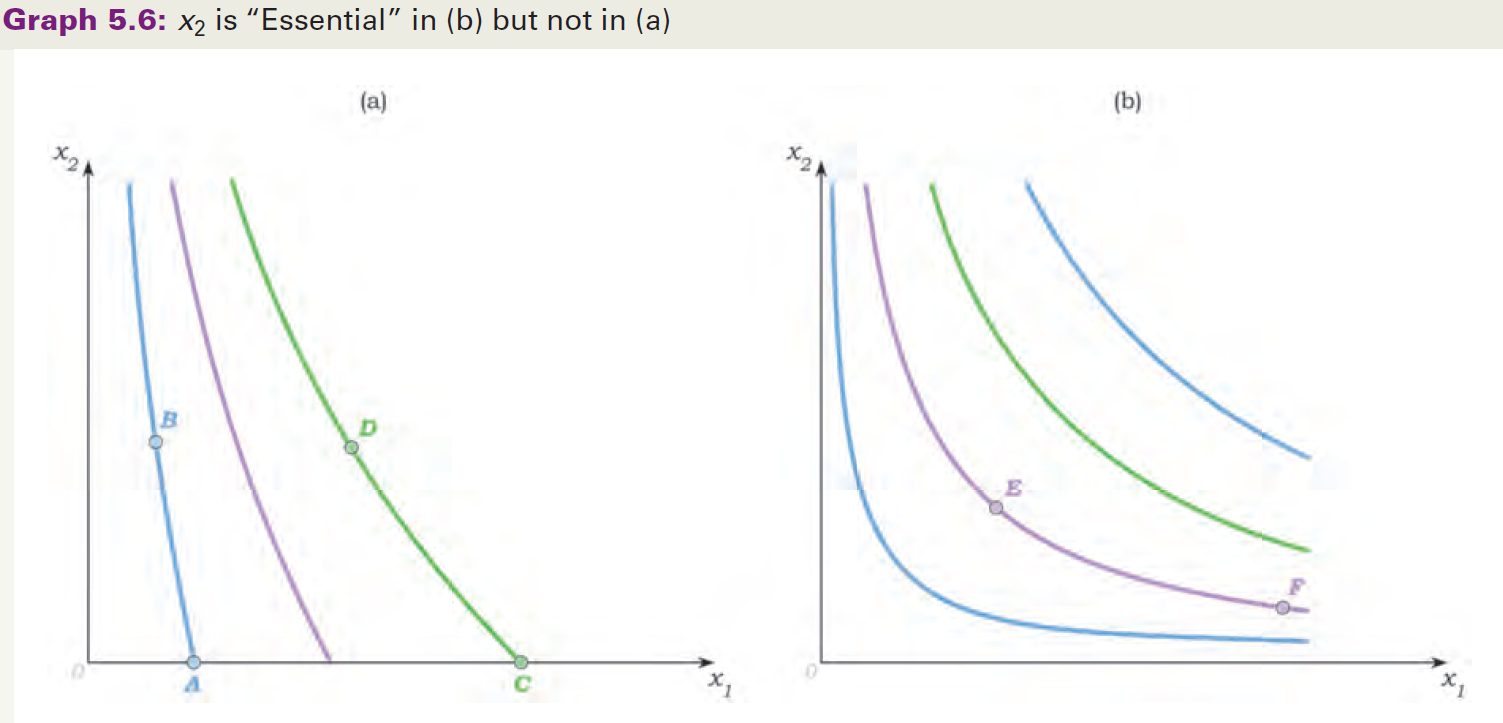
\includegraphics[width=1\textwidth]{5_1} %插入图片,[]中设置图片大小,{}中是图片文件名
	\caption{} %最终文档中希望显示的图片标题
	\label{Fig.main2} %用于文内引用的标签
\end{figure}

若无差异曲线与$ x_2 $轴相交,则可以实现在$ x_1 $为零的情况下比原点更好的商品束,在这种意义上,$ x_1 $是不必要的,反之若不能与$ x_2 $轴相交,则$ x_1 $是必要的。

若在某种偏好下所有商品束都是必要的,则一般不存在角点解。
(一般是指在常见预算约束下,在某些预算约束下还是可以存在角点解,例如配额,网课有讲)。





\end{document}